\subsection{Method}

In this second section of the second part, we describe the developed solution to the problem introduced hereinabove, with an overview of the software implementation of the project.
We mainly present the proposed DQN model; DQN-ITSCwPD (DQN Intelligent Traffic Signal Control with Partial Detection). We also detail the customized environment implemented with the Sumo traffic simulator, and two  algorithms as comparison baselines. 

\subsubsection{Environment implementation}

\textbf{Customized environment in frameworQ} \\
As mentioned before, the application project is implemented within frameworQ, the DQN framework for customized environments (see part 1.3). Hence, only the customized environment is added in the \texttt{env/} package, with the rest of the architecture left unchanged. The environment model encompasses a Traci interface for traffic signal control in the Sumo traffic simulator, and the corresponding Sumo configuration files, as well as the DQN controller and additional resources. An installation script is provided to build the project and its dependencies, with the \texttt{sumo} software as a local \texttt{venv/} package, at \texttt{bin/make.sh}. \\

\textbf{Sumo simulation configuration data} \\
In the Sumo traffic simulator, simulation scenarios are defined by \texttt{XML} configuration data files. In the project environment, a \texttt{data/} folder contains these \texttt{XML} configuration data files, with one sub-folder per simulation scenario. A \texttt{.net.xml} file, created with the \texttt{netedit} visual network editor, configures the network, with the approaches, lanes and connections for all the roads and intersections. A \texttt{.tll.xml} file configures the traffic signal logic, with the programs of the traffic lights in the network. The programs contain all the possible phases, which are represented as the sequences of signals over a complete clockwise rotation around an intersection. A \texttt{.rou.xml} file configures the route definitions, i.e. the possible itineraries in the network, and the traffic demand over these itineraries. It first lists the routes as the sequences of their consecutive approaches, then the types of vehicles that can be inserted in the network, and finally the traffic demand for the simulation as all the individual vehicles to be inserted, by time of insertion in the network and with their respective itineraries. Contrary to the two previous configuration files that are fixed, the route configuration file is intended to change between simulations as the traffic demand vary. A \texttt{.sumocfg} file serves as an entry point to the simulator for a given simulation scenario, by grouping the paths to the aforementioned configuration files. Finally, an optional \texttt{gui-settings.cfg} file configures the visual settings for the graphical interface \texttt{sumo-gui}. \\

\textbf{Sumolib-Traci interface for Sumo TSC} \\
Sumo provides two python tools for interfacing the traffic simulator. The \texttt{sumolib} library provides a set of static methods to parse configuration files and retrieve network structural information. The \texttt{traci} library provides a set of methods to interact dynamically with the simulated objects in real time, both to retrieve and to modify data online. Both tools are used in the \texttt{sumo\_env.py} file, a Sumo traffic signal control interface. As the DQN model is intended to be run on a wider range of traffic situations, the interface is designed to be flexible towards parameterized traffic scenario loading and traffic demand generation, and thus contains no hard coded information. The simulations are handled by a two-step process, with an initial mapping procedure and episodic traffic demand generation. At each episode, a simulation is started and run on a \texttt{traci} sub-process from the configuration files in the corresponding \texttt{data/} sub-folder, with either \texttt{sumo} or \texttt{sumo-gui}. \\ 

\textbf{Initialization mapping procedure} \\
In the \texttt{sumolib-traci} TSC interface, an initial mapping procedure enables to dynamically load new traffic scenarios from a \texttt{data/} sub-folder without hard coded information, prior to starting the first simulation. Firstly, the road network is parsed with \texttt{sumolib} to create two structural maps. The map of intersections with traffic lights is recovered, along with their respective maps of incoming and outgoing approaches and lanes. The map of possible routes is generated by applying the Dijkstra path finding algorithm between all combinations of entry and exit approaches in the network. Secondly, an empty simulation, that is with no traffic demand and killed instantly, is launched with \texttt{traci} to create the map of traffic signal logic. This, by completing a full cycle of phases for every traffic light programs, along with their respective maps of green interval signals and open connections. \\

\textbf{Episode traffic demand generation} \\
In the \texttt{sumolib-traci} TSC interface, new traffic demand is generated at each simulation, i.e. each episode, to create unseen traffic situations for the DQN agent. At each episode, each entry approach $e$ in the network is assigned an insertion traffic flow $q_e$, in vehicles per hour. From these traffic flows, traffic demand is generated for each entry approach by a Poisson process with rate $\lambda_e = q_e^{-1}\cdot 3600$ over the duration of the simulation. For each entry approach, the vehicles are randomly distributed over the connections of the intersection, such that the insertion traffic flow is proportionally split over the possible routes. Each episode is also assigned a CV penetration rate $p_{cv}$, and a proportion of $p_{cv}$ vehicles are identified as connected, while the complementary proportion of $1-p_{cv}$ vehicles are identified as conventional. The total traffic demand is sorted by insertion time in the simulation, and written to the \texttt{.rou.xml} route configuration file, with the corresponding routes listed in the initialization mapping procedure and special vehicle types for CV and non-CV. The insertion traffic flows $q_e$ and the CV penetration rate $p_{cv}$ can either be set manually as hyper-parameters, or be chosen randomly at each episode of simulation. \\

\textbf{Scheduler for multiple TL control} \\
The timesteps experienced by the DQN agent as part of the decision making problem do not coincide with the internal clock refresh rate in the simulation, that is every second. Moreover, a delay is introduced between the decision to change phase and the actual phase change, as the phase transition between two green intervals goes through intermediate change and clearance intervals. Finally, in a traffic scenario with multiple intersections, this delay can induce overlaps between the time intervals over the different traffic lights. \\
We introduce a special data structure for scheduling phase changes in \texttt{
tl\_scheduler.py}, to counter these problems. This traffic light scheduler stores the upcoming phase changes planned for each traffic light, and effectively performs these transitions with respect to the green, change and clearance intervals. The adequate number of internal transitions are completed in the simulator and abstracted from the DQN agent, which is called only upon decision making. Thus, this scheduling data structure enables to control multiple traffic lights without time interference, despite centralized transition dynamics in Sumo.

\subsubsection{DQN-ITSCwPD model}

\textbf{DQN control with Per3DQN+} \\
As mentioned before and as part of frameworQ, traffic signal control is conducted with the Per3DQN+ algorithm (see part 1.3.2). We present here the proposed DQN model; DQN-ITSCwPD (DQN Intelligent Traffic Signal Control with Partial Detection), i.e. the action, observation and reward functions, the neural network and the hyper-parameters. The three former are implemented in \texttt{rl\_controller.py}, inherited from \texttt{sumo\_env.py} with \texttt{traci} and encapsulated in \texttt{dqn\_env.py}, and the two latter are defined in \texttt{dqn\_config.py}.\\

\textbf{Action: phase selection} \\
The agent selects the next phase for the next $T_g$ seconds of green time interval among the set of all possible phases, at a given traffic light. If the selected phase is the same as the current phase, the current green interval is extended by $T_g$ seconds. Else, a transition to the next phase is executed, with an intermediate $T_y + T_r$ seconds through change and clearance intervals, and an initial $T_g$ seconds in the green interval of the selected phase. Thus, while the action is formally to select the next phase, the agent also indirectly decides the duration of the current phase by selecting the same phase multiple times consecutively. \\

\textbf{Action space: size 2 or 4} \\ 
The action space is defined by the number of possible phases in the traffic light program. At a four-way intersection, there is a total of 8 valid paired signal phases for non-conflicting movement signals [34]. From this, the set of possible phases, i.e. with no or minimum conflicts, has either 2, 4 or 8 phases, and are as follows with their respective action spaces:
\begin{itemize}
\setlength\itemsep{-0.5em}
  \item \textbf{2 phases}: 2-phases programs are used for small intersections and traffic flows, with conflicting left turns authorized. They have two permissive green intervals, one for each axis, with permissive turn left, through and turn right movements. The first phase, along the north-south axis, is (1) from north to east, south and west, and from south to west, north and east. The second phase, along the east-west axis, is (2) from east to south, west and north, and from west to north, east and south. The action space is $A=\{(n\rightarrow esw,s\rightarrow wne),(e\rightarrow swn,w\rightarrow nes)\}$, with size $|A|=2$.
  \begin{figure}[h]
    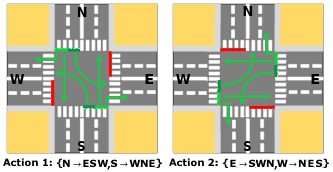
\includegraphics[scale=0.8]{img/II/2phases.png}
    \centering
    \captionsetup{justification=centering}
    \caption{2 phases, action space.}
  \end{figure}
  \item \textbf{4 phases}: 4-phases programs are used over medium to large intersections and traffic flows, with protected left turns only. They have four protected green intervals, two for each axis, with protected turn left movements only, or through and turn right movements. The first and second phases, along the north-south axis, are (1) from north to south and west, and from south to north and east, and (2) from north to east, and from south to west. The third and fourth phases, along the east-west axis, are (3) from east to west and north, and from west to east and south, and (4) from east to south, and from west to north. The action space is $A=\{(n\rightarrow sw,$ $s\rightarrow ne),(n\rightarrow e,s\rightarrow w),(e\rightarrow wn,w\rightarrow es),(e\rightarrow s,w\rightarrow n)\}$, with size $|A|=4$.
  \begin{figure}[h]
    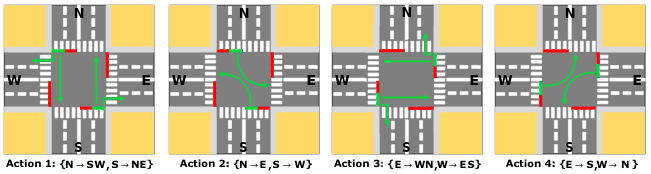
\includegraphics[scale=0.8]{img/II/4phases.png}
    \centering
    \captionsetup{justification=centering}
    \caption{4 phases, action space.}
  \end{figure}
  \item \textbf{8 phases}: 8-phases programs are used rarely in practice, and are not studied here.
\end{itemize}

\textbf{Observation: partial DTSE} \\
Discrete traffic state encoding (DTSE) [20] (Gao et al., 2017) is a microscopic, image-like state representation of the intersection for TSC. Here, we adapt DTSE to the partially observed environment with detection on connected vehicles, and propose partial DTSE.

\pagebreak

\newgeometry{left= 3cm, right= 2cm, bottom= 0cm, top= 2.6cm}

In partial DTSE, the state representation is an image-like construction of stacked 2D-matrices for multiple levels of microscopic, individual information provided by connected vehicles and traffic signals at the intersection. Here, all incoming lanes are discretized, over segments from the stop line up to a detection range less than or equal to the total length of the corresponding approach, into grids with cells of fixed length, set to be slightly larger than the average size of a vehicle with inter-vehicle gap. The cells contain data on individual CVs and traffic signals, and the grids are aggregated over the segments. Three 2D-matrices are extracted for three levels of information; i.e. the matrix of CV positions $P$, the matrix of CV speeds $V$, and the matrix of traffic signals over lanes $S$; and stacked into a single image-like state representation of the intersection; partial DTSE: \\
\[ \text{Partial DTSE} = \{P = [P_0, P_1, P_2, P_3]; V = [V_0, V_1, V_2, V_3]; S = [S_0, S_1, S_2, S_3] \} \]

\begin{figure}[h]
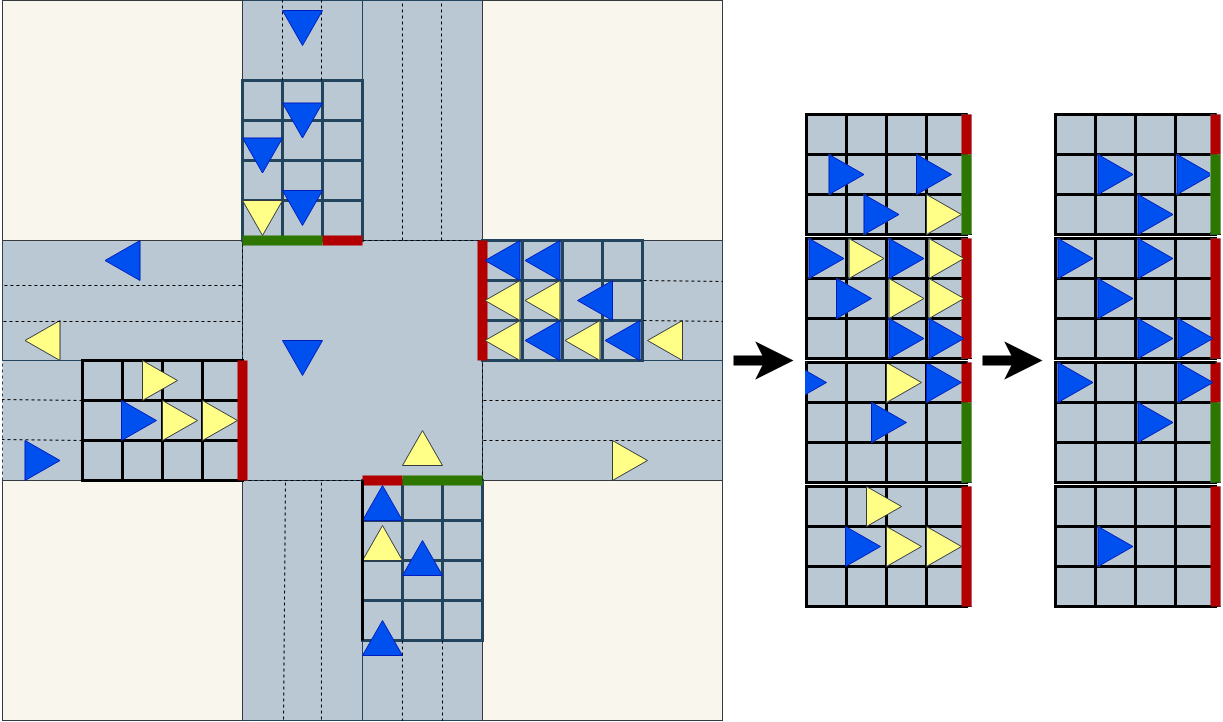
\includegraphics[width=\textwidth]{img/II/pdtse_full.png}
\centering
\end{figure}

\begin{table}[!htbp]
\centering
\setlength\tabcolsep{2pt}
\begin{tabular}{c}
Partial DTSE = 
\end{tabular}
\begin{tabular}{|c|c|c|c|}
\hline
\multicolumn{4}{|c|}{$P = [P_0, P_1, P_2, P_3]$} \\
\hline
\:\: 0 \:\: & \:\: 0 \:\: & \:\: 0 \:\: & \:\: 0 \:\: \\ \hline
\:\: 0 \:\: & \:\: 1 \:\: & \:\: 0 \:\: & \:\: 1 \:\: \\ \hline
\:\: 0 \:\: & \:\: 0 \:\: & \:\: 1 \:\: & \:\: 0 \:\: \\ \hline
\:\: 1 \:\: & \:\: 0 \:\: & \:\: 1 \:\: & \:\: 0 \:\: \\ \hline
\:\: 0 \:\: & \:\: 1 \:\: & \:\: 0 \:\: & \:\: 0 \:\: \\ \hline
\:\: 0 \:\: & \:\: 0 \:\: & \:\: 1 \:\: & \:\: 1 \:\: \\ \hline
\:\: 1 \:\: & \:\: 0 \:\: & \:\: 0 \:\: & \:\: 1 \:\: \\ \hline
\:\: 0 \:\: & \:\: 0 \:\: & \:\: 1 \:\: & \:\: 0 \:\: \\ \hline
\:\: 0 \:\: & \:\: 0 \:\: & \:\: 0 \:\: & \:\: 0 \:\: \\ \hline
\:\: 0 \:\: & \:\: 0 \:\: & \:\: 0 \:\: & \:\: 0 \:\: \\ \hline
\:\: 0 \:\: & \:\: 1 \:\: & \:\: 0 \:\: & \:\: 0 \:\: \\ \hline
\:\: 0 \:\: & \:\: 0 \:\: & \:\: 0 \:\: & \:\: 0 \:\: \\ \hline
\end{tabular}
\begin{tabular}{|c|c|c|c|}
\hline
\multicolumn{4}{|c|}{$V = [V_0, V_1, V_2, V_3]$} \\
\hline
\:\: 0 \:\: & \:\: 0 \:\: & \:\: 0 \:\: & \:\: 0 \:\: \\ \hline
\:\: 0 \:\: & 0.9 & \:\: 0 \:\: & 0.8 \\ \hline
\:\: 0 \:\: & \:\: 0 \:\: & 0.8 & \:\: 0 \:\: \\ \hline
\:\: 0 \:\: & \:\: 0 \:\: & \:\: 0 \:\: & \:\: 0 \:\: \\ \hline
\:\: 0 \:\: & 0.2 & \:\: 0 \:\: & \:\: 0 \:\: \\ \hline
\:\: 0 \:\: & \:\: 0 \:\: & \:\: 0 \:\: & \:\: 0 \:\: \\ \hline
0.4 & \:\: 0 \:\: & \:\: 0 \:\: & \:\: 0 \:\: \\ \hline
\:\: 0 \:\: & \:\: 0 \:\: & 0.7 & \:\: 0 \:\: \\ \hline
\:\: 0 \:\: & \:\: 0 \:\: & \:\: 0 \:\: & \:\: 0 \:\: \\ \hline
\:\: 0 \:\: & \:\: 0 \:\: & \:\: 0 \:\: & \:\: 0 \:\: \\ \hline
\:\: 0 \:\: & 0.1 & \:\: 0 \:\: & \:\: 0 \:\: \\ \hline
\:\: 0 \:\: & \:\: 0 \:\: & \:\: 0 \:\: & \:\: 0 \:\: \\ \hline
\end{tabular}
\begin{tabular}{|c|c|c|c|}
\hline
\multicolumn{4}{|c|}{$S = [S_0, S_1, S_2, S_3]$} \\
\hline
\:\: 0 \:\: & \:\: 0 \:\: & \:\: 0 \:\: & \:\: 0 \:\: \\ \hline
\:\: 1 \:\: & \:\: 1 \:\: & \:\: 1 \:\: & \:\: 1 \:\: \\ \hline
\:\: 1 \:\: & \:\: 1 \:\: & \:\: 1 \:\: & \:\: 1 \:\: \\ \hline
\:\: 0 \:\: & \:\: 0 \:\: & \:\: 0 \:\: & \:\: 0 \:\: \\ \hline
\:\: 0 \:\: & \:\: 0 \:\: & \:\: 0 \:\: & \:\: 0 \:\: \\ \hline
\:\: 0 \:\: & \:\: 0 \:\: & \:\: 0 \:\: & \:\: 0 \:\: \\ \hline
\:\: 0 \:\: & \:\: 0 \:\: & \:\: 0 \:\: & \:\: 0 \:\: \\ \hline
\:\: 1 \:\: & \:\: 1 \:\: & \:\: 1 \:\: & \:\: 1 \:\: \\ \hline
\:\: 1 \:\: & \:\: 1 \:\: & \:\: 1 \:\: & \:\: 1 \:\: \\ \hline
\:\: 0 \:\: & \:\: 0 \:\: & \:\: 0 \:\: & \:\: 0 \:\: \\ \hline
\:\: 0 \:\: & \:\: 0 \:\: & \:\: 0 \:\: & \:\: 0 \:\: \\ \hline
\:\: 0 \:\: & \:\: 0 \:\: & \:\: 0 \:\: & \:\: 0 \:\: \\ \hline
\end{tabular}
    \captionsetup{justification=centering}
    \captionof{figure}{Partial DTSE.}
\end{table}

\restoregeometry

\pagebreak

The above example demonstrates partial DTSE applied to a four-way intersection, with connected vehicles in blue and conventional vehicles in yellow. The matrix of CV positions $P$ is binary encoded, with 1 and 0 being respectively the presence or absence of connected vehicles in the cells. The matrix of CV speeds $V$ encodes the corresponding speeds, normalized over the speed limits of approaches. The matrix of traffic signals over lanes $S$ is binary encoded, with 1 being a green signal for the lane and 0 another signal.
In Sumo, the vehicle size and inter-vehicle gap are 5 and 2.5 meters. Thus, we use cells of 8 meters, and a detection range of 160 meters, i.e. sensing up to twenty CVs per lane. \\

\textbf{Reward: total squared delay} \\
The goal of the agent is to minimize the total travel time through the intersection for all commuters, i.e. for both connected and conventional vehicles. As such, while the state represents only CVs in a partially observed environment, the reward function considers all vehicles in a fully observed environment. This implies that full training is completed in the simulator, where conventional vehicles are observable, and performances do not improve after deployment [30]. We propose a reward function based on vehicle delay, as delay was considered the most efficient metric for learning by a comparative study [33]. Minimizing delay translates to minimizing the lost travel time $\overline{t} - t_{min}$, with $\overline{t}$ the average travel time of vehicles and $t_{min}$ the lowest possible travel time with speed limit $v_{max}$ [30]. Over the travel distance $t_{min} \cdot v_{max}$, for a given vehicle $i$ with speed $v_i(t)$, and at time $t$:

\[ t_{min} \cdot v_{max} = \int_{0}^{\overline{t}} v_i(t) \,dt \implies t_{min} = \frac{1}{v_{max}} \int_{0}^{\overline{t}} v_i(t) \,dt \]

\[ \implies \overline{t} - t_{min} =  \int_{0}^{\overline{t}} 1 \,dt - \frac{1}{v_{max}} \int_{0}^{\overline{t}} v_i(t) \,dt = \frac{1}{v_{max}} \int_{0}^{\overline{t}} v_{max} - v_i(t) \,dt \]
\\
Thus, minimizing the delay is equivalent to minimizing, for each timestep $t$ and vehicle $i$:

\[ d_i(t) = \frac{1}{v_{max}} \cdot ({v_{max}} - v_i(t)) = 1 - \frac{v_i(t)}{v_{max}} \]
\\
The goal is to decrease the delay for all vehicles, and we hence use a cumulative metric. Total delay is preferred over average delay, as it retains information on the volume of vehicles at the intersection. Moreover, we apply a power term so that fewer large delays are prioritized over many short delays, which encourages fairness between vehicles. Besides, exponents in reward functions are empirically known to boost learning, as they emphasize small performance gains towards the objective. Thus, we present the total squared delay:
\[ tsd(t) = \sum_{i} (1 - (\frac{v_i(t)}{v_{max}})^2) \]

\pagebreak

\newgeometry{left= 3cm, right= 2cm, bottom= 0cm, top= 2.6cm}

As rewards are maximized, minimizing a metric equates to maximizing its negated value. Here, the reward function acts in effect as a punishment, by maximizing the negative total squared delay. Additionally, the reward is normalized by the maximum total squared delay encountered at that time of training $tsd_{max}(t) = \max (tsd(t), tsd_{max}(t-1))$, and centered in $[0, 1]$ for learning stability [18]. Thus, the complete TSC reward function is given by:
\[ r(t) = 1 - \frac{tsd(t)}{tsd_{max}(t)} = 1 - \frac{\sum_{i} (1 - (\frac{v_i(t)}{v_{max}})^2)}{\max (tsd(t), tsd_{max}(t-1))}\]
\\
\textbf{Convolutional NN, hyper-parameters} \\
The convolutional neural network (CNN) [36] (Krizhevsky et al., 2012) is a special NN architecture for image analysis. The underlying principles of forward and back propagation apply as presented earlier, but the architecture is split into two distinct learning modules. \\
A first learning module, the convolutional module, is composed of convolutional layers, that assemble patterns of increasing complexity in data with space invariant operations. They perform 2D-convolutions over shared weights of filters, or kernels, sliding with a stride along stacked input feature 2D-matrices called channels, to output feature maps. Additionally, optional intermediate pooling layers reduce the dimensions of the feature maps. Thus, a convolutional layer is defined by a number of channels $C$, a kernel size $K$ and a stride $S$. The output from the last convolutional layer is flattened and passed to a second learning module, the fully connected module, a MLP with fully connected layers. \\
Here, partial DTSE is a 3-channels image-like state representation with cells acting as pixels, and thus a convolutional dueling DQN maps from partial DSTE observations to phase selection actions. After experiments, we shaped the CNN to have two convolutional layers and two fully connected layers; i.e. $CNN1$ with $(C=16,K=4,S=2)$, $CNN2$ with $(C=32,K=2,S=1)$, $FC1$ with $128$ neurons and $FC2$ with $64$ neurons. Adding the input, dueling and aggregation output layers, the convolutional dueling DQN is as follows: \\

\begin{figure}[h]
  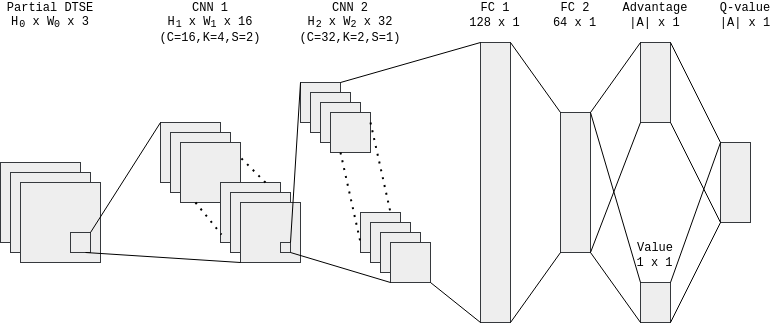
\includegraphics[width=\textwidth]{img/II/cnn_dueling.png}
  \centering
  \captionsetup{justification=centering}
  \caption{Convolutional dueling DQN.}
\end{figure}

\restoregeometry

\pagebreak

The model was tuned by grid search over the hyper-parameters, with tuning runs set to $200000$ timesteps. The tuned hyper-parameters are $\alpha=\num{1e-4}$ with Adam optimizer and Huber loss, $\gamma=0.99$, $\epsilon_{min}=0.01$, $\epsilon_{dec}=2$M with exponential decay, $N=1$M, $N_{min}=0.1$M, $\tau=\num{1e-3}$ with soft Polyak update. No terminal state is defined for the agent, and episodes are early stopped by an internal time limit in the Sumo simulation.

\subsubsection{Comparison baselines}

\textbf{Actuated TSC baselines}\\
Actuated traffic signal controllers are adaptive, non-learning TSC algorithms, responding to traffic flows in real time by measuring requests for green signals over the competing phases, according to fixed rules [34]. They rely on full, macroscopic traffic detection and are already extensively deployed at real intersections with inductive loops under the roads. 
As there exist, for the time being, no standard algorithm for deep Q-learning TSC with partial detection, neither deployed nor in the literature, we compare the proposed model to two actuated TSC algorithms; i.e. Max Pressure and SOTL [18]. These comparison baselines are implemented in \texttt{baselines.py}, inherited from \texttt{sumo\_env.py} with \texttt{traci}. \\

\textbf{Max Pressure}\\
Max Pressure (Varaiya, 2013) [37] is an acyclic actuated TSC algorithm which minimizes the pressure of phases at an intersection. The pressure of a phase $p$ at an intersection is defined as the difference between the total number of vehicles in the set of all incoming lanes with authorized movements for that phase $L_{p,inc}$ and the total number of vehicles in the set of all corresponding outgoing lanes $L_{p,out}$; i.e. $pressure(p) = \sum_{l \in L_{p,inc}} |V_l| - \sum_{l \in L_{p,out}} |V_l|$. \\
After each green interval of time $T_g$, the controller selects the phase $p \in P$ with maximum pressure to be relieved in the set of all possible phases. If the selected phase is the same as the current phase, the current green interval is extended by $T_g$ seconds. Else, a transition to the next phase is executed, with an intermediate $T_y + T_r$ seconds through change and clearance intervals, and an initial $T_g$ seconds in the green interval of the selected phase. While Max Pressure is an efficient and simple to implement actuated TSC algorithm, it presents a major drawback as it involves detection on vehicles in both incoming and outgoing lanes, and thus requires twice as much infrastructure and cost at real intersections. \\

\textbf{SOTL}\\
Self-organizing traffic lights (SOTL) (Gershenson, 2004) [38] is a cyclic actuated TSC algorithm which dynamically sets the green interval duration $T_g$ in the current phase $p$. \\
(1) A time integral $\kappa$ of the total number of vehicles in the set of all incoming lanes with prohibited movements for that phase $L_{inc} - L_{p,inc}$ and in a distance $\psi$ from the stop line is accumulated, and the current phase is maintained until the accumulated time integral reaches a fixed threshold $\theta$; i.e. $T_g$ = $T_g+1$, while $\kappa \le \theta$, with $\kappa = \kappa + \sum_{l \in L_{inc} - L_{p,inc}} |V_{l,\psi}|$.
(2) In addition to (1), small vehicle platoons of size $n$, the total number of vehicles in the set of all incoming lanes with authorized movements for that phase $L_{p,inc}$ and in a distance $\omega \le \psi$ from the stop line, are kept together and prevent phase changes for sizes less than a fixed threshold $\mu$; i.e. $T_g$ = $T_g+1$, if $0 < n \le \mu$, with $n = \sum_{l \in L_{p,inc}} |V_{l,\omega}|$.
According to (1) and (2), else, a transition to the next phase is executed, with an intermediate $T_y + T_r$ seconds through change and clearance intervals, and an initial $T_g$ seconds in the green interval of the next phase $p \in P$ in the cycle. Here, the constants are set to values commonly found in the literature; i.e. $\theta = 50$, $\mu = 3$, and $\psi = 80$, $\omega = 25$ meters. \\

\textbf{Algorithms}\\
The pseudo codes presented hereinafter are highly summarized, and do not include the phase transition procedure, nor the TL scheduling and the integration of Sumo dynamics. \\

\begin{algorithm}[H]
\small
\caption*{Max Pressure algorithm}
\begin{algorithmic}
    \IF{$T_g \ge T_{g,min}$}
        \STATE Set the next phase to maximum pressure phase $p = arg\max(\{pressure(p) \textbf{ for } p \in P\})$
        \STATE with $pressure(p) = \sum_{l \in L_{p,inc}} |V_l| - \sum_{l \in L_{p,out}} |V_l|$;
    \ENDIF
\end{algorithmic}
\end{algorithm}

\begin{algorithm}[H]
\small
\caption*{SOTL algorithm}
\begin{algorithmic}
    \STATE Accumulate the time integral $\kappa = \kappa + \sum_{l \in L_{inc} - L_{p,inc}} |V_{l,\psi}|$;
    \IF{$T_g \ge T_{g,min} \textbf{ and } \kappa > \theta$}
        \STATE Set the vehicle platoon size $n = \sum_{l \in L_{p,inc}} |V_{l,\omega}|$;
        \IF{$n \text{ null  }\textbf{ or } n > \mu$}
            \STATE Set $\kappa = 0$;
            \STATE Set the next phase to the next phase in the cycle $p \in P$;
        \ENDIF
    \ENDIF
\end{algorithmic}
\end{algorithm}

\pagebreak
